\documentclass[border=10pt]{standalone}
\usepackage{tikz}
\usetikzlibrary{shapes.geometric,shapes.symbols,arrows.meta,positioning}

\begin{document}
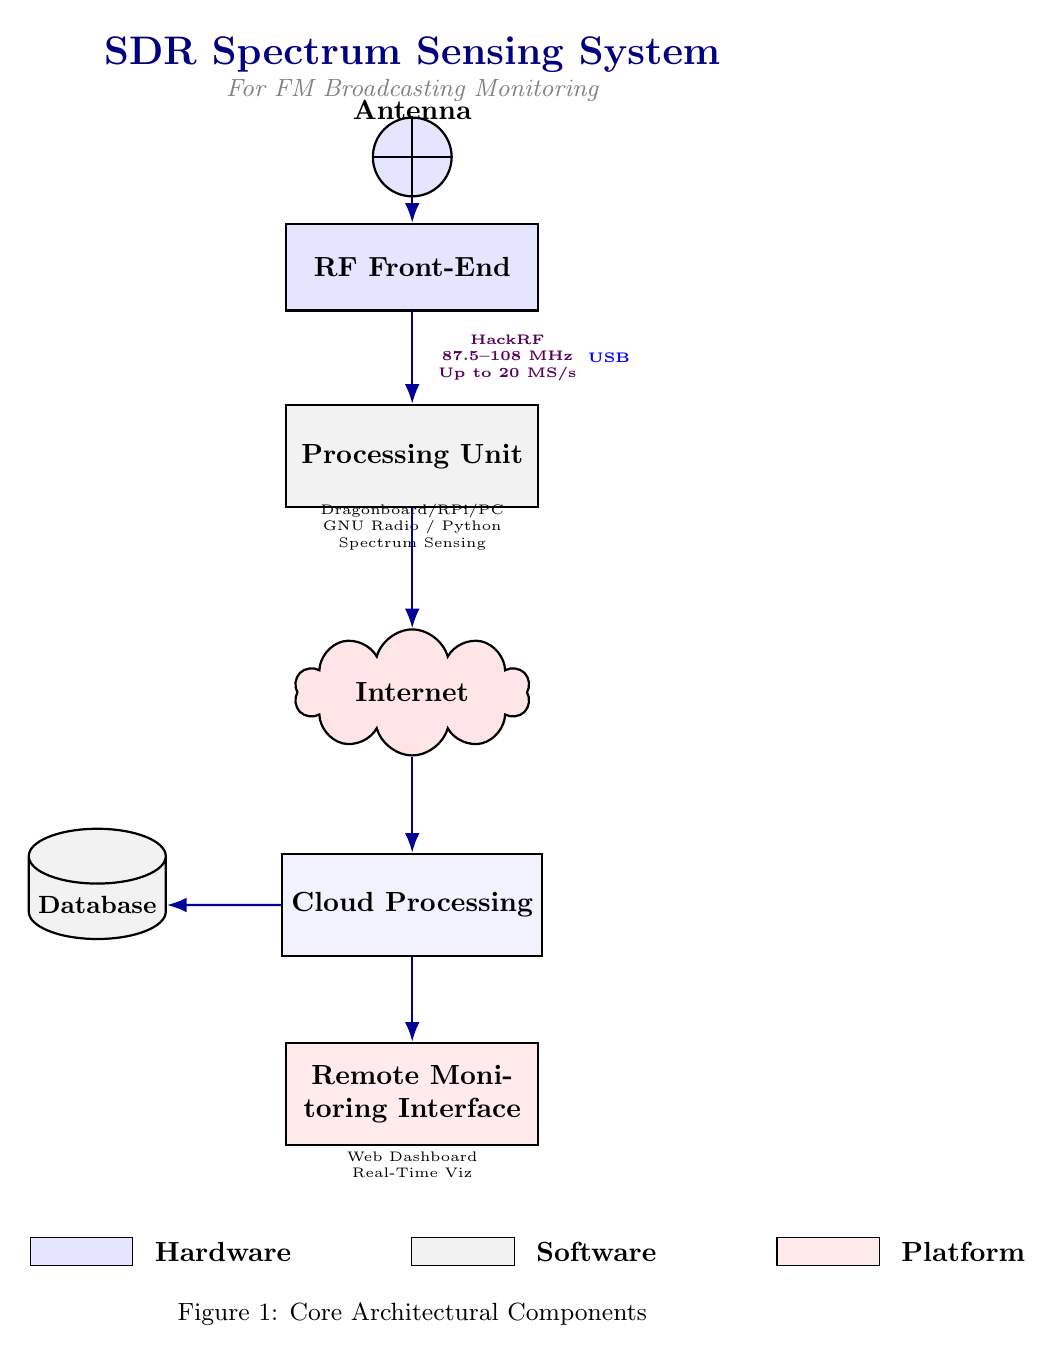
\begin{tikzpicture}[
    font=\small,
    box/.style={rectangle, draw=black, thick, minimum width=3.2cm, minimum height=1.1cm,
                align=center, font=\bfseries},
    hwbox/.style={box, fill=blue!10},
    swbox/.style={box, fill=black!5},
    platbox/.style={box, fill=red!8},
    cyl/.style={cylinder, shape border rotate=90, draw=black, thick, fill=black!5,
                minimum width=1.6cm, minimum height=1.4cm, aspect=0.4, align=center, font=\bfseries\small},
    cloudshape/.style={cloud, draw=black, thick, fill=red!10, aspect=2,
                        minimum width=3cm, minimum height=1.6cm, align=center},
    arr/.style={-{Latex[length=2.5mm]}, thick, blue!60!black},
    lbl/.style={font=\tiny\bfseries, align=center, text=violet!70!black}
]

% ---- Title ----
\node[align=center, blue!50!black] at (0,9.4) {\Large\bfseries SDR Spectrum Sensing System};
\node[align=center, gray] at (0,8.95) {\itshape For FM Broadcasting Monitoring};

% ---- Antenna ----
\node[circle, draw=black, thick, fill=blue!10, minimum size=1cm] (antenna) at (0,8.1) {};
\draw[thick] (antenna.north) -- ++(0,-1);
\draw[thick] (antenna.south) -- ++(0,1);
\draw[thick] (antenna.west) -- ++(1,0);
\draw[thick] (antenna.east) -- ++(-1,0);
\node[font=\bfseries] at (0,8.7) {Antenna};

% ---- RF Front-End ----
\node[hwbox] (rf) at (0,6.7) {RF Front-End};
\draw[arr] (antenna.south) -- (rf.north);

% ---- Processing Unit ----
\node[swbox, minimum height=1.3cm] (proc) at (0,4.3) {Processing Unit};
\draw[arr] (rf.south) -- (proc.north)
    node[midway, right, lbl, xshift=2mm] {HackRF\\87.5--108 MHz\\Up to 20 MS/s};
\node[lbl, blue] at (2.5,5.55) {USB};
\node[align=center, font=\tiny] at (0,3.4) {Dragonboard/RPi/PC\\GNU Radio / Python\\Spectrum Sensing};

% ---- Internet cloud (between Processing Unit and Cloud Processing) ----
\node[cloudshape] (net) at (0,1.3) {};
\node[font=\bfseries] at (0,1.3) {Internet};
\draw[arr] (proc.south) -- (net.north);

% ---- Cloud Processing (new) ----
\node[swbox, minimum height=1.3cm, fill=blue!5] (cloud) at (0,-1.4) {Cloud Processing};
\draw[arr] (net.south) -- (cloud.north);

% ---- Database (now attached to Cloud Processing) ----
\node[cyl] (db) at (-4,-1.4) {Database};
\draw[arr] (cloud.west) -- (db.east);

% ---- Remote Monitoring Interface ----
\node[platbox, minimum height=1.3cm] (mon) at (0,-3.8) {Remote Moni-\\toring Interface};
\draw[arr] (cloud.south) -- (mon.north);
\node[align=center, font=\tiny] at (0,-4.7) {Web Dashboard\\Real-Time Viz};

% ---- Legend ----
\node[rectangle, draw=black, fill=blue!10, minimum width=1.3cm, minimum height=0.35cm] (leg1) at (-4.2,-5.8) {};
\node[right=0.15cm of leg1, font=\bfseries] (leg1txt) {Hardware};

\node[rectangle, draw=black, fill=black!5, minimum width=1.3cm, minimum height=0.35cm, right=1.4cm of leg1txt] (leg2) {};
\node[right=0.15cm of leg2, font=\bfseries] (leg2txt) {Software};

\node[rectangle, draw=black, fill=red!8, minimum width=1.3cm, minimum height=0.35cm, right=1.4cm of leg2txt] (leg3) {};
\node[right=0.15cm of leg3, font=\bfseries] {Platform};

% ---- Caption ----
\node[align=center] at (0,-6.6) {Figure 1: Core Architectural Components};

\end{tikzpicture}
\end{document}
